\chapter{Trabalhos Relacionados}
% * <profsean@gmail.com> 2017-01-18T20:19:34.451Z:
% 
% > Trabalhos
% Independente de juntar ou não os capítulos, é importante encadear esta parte do texto com a anterior... Ficou uma quebra... muda completamente de assunto...
% 
% ^.
\label{cap:relacionados}
Neste capítulo serão apresentadas duas ferramentas para o alinhamento de dados conectados. As ferramentas apresentadas a seguir foram selecionadas devido ao seu destaque na edição de 2016 do relatório publicado pela Ontology Alignment Evaluation Initiative (OAEI). Inicialmente, a OAEI avaliava apenas ferramentas de alinhamento de ontologias, dando início à avaliação de soluções para alinhar dados em 2009. Desde então, um número crescente aplicações vêm sendo submetidas.
% * <profsean@gmail.com> 2017-01-18T20:22:17.708Z:
% 
% > Desde então, um número crescente aplicações vêm sendo submetidas
% Dados que comprovem? Evidências disto?
% 
% ^.
% * <profsean@gmail.com> 2017-01-18T20:21:19.611Z:
% 
% > devido ao seu destaque
% Deveria explicar melhor que destaque foi esse...
% 
% ^.

\section{AgreementMakerLight (AML)}
Desenvolvido em parceria entre o Instituto Gulbenkian de Ciência, a Universidade de Lisboa, e a Universidade de Illinois, o AgreementMakerLight é uma ferramenta de alinhamento de ontologias. De acordo com \cite{fariaoaei}, o AML se baseia inicialmente em técnicas e similaridade léxica, tendo como ênfase o uso de fontes externas como \textit{background}.

O AML conta com três algoritmos para alinhamento voltados a correspondência de instâncias, sendo eles o \textit{HybridStringMatcher}, o \textit{ValueStringMatcher} e o \textit{Value2LexiconMatcher}. O primeiro utiliza diversas abordagens para gerar a similaridade, sendo elas a comparação entre frases, palavras. Além disso, essa abordagem hibrida também explora a \textit{WordNet}. O segundo utiliza o mapeamento de valor para gerar calcular a similaridade, penalizando pares nos quais anotações ou propriedades de dados não são os mesmos. Por fim, o terceiro une as duas abordagens anteriores.

Apesar do AML possuir diferentes algoritmos de alinhamento na ferramenta, todos eles trabalham apenas no nível dos dados. Consequentemente, as características das propriedades são desconsideradas ao longo do processo de correspondência.

\section{RiMOM-2016}
Baseando-se no RiMOM  \cite{li2009rimom}, \citeonline{zhang2016rimom} desenvolveram o RiMOM-2016, que é uma ferramenta para alinhar dados conectados. Ela implementa um número considerável de abordagens para alinhar, cuja escolha é realizada através dos metadados extraídos da ontologia. Além disso, o RiMOM-2016 utiliza um índice invertido para indexar os objetos e consequentemente gerar pares candidatos para um possível alinhamento. A geração dos pares é realizada quando dois recursos compartilham pelo menos um predicado e objeto.

\begin{figure}[!ht]
	\centering
	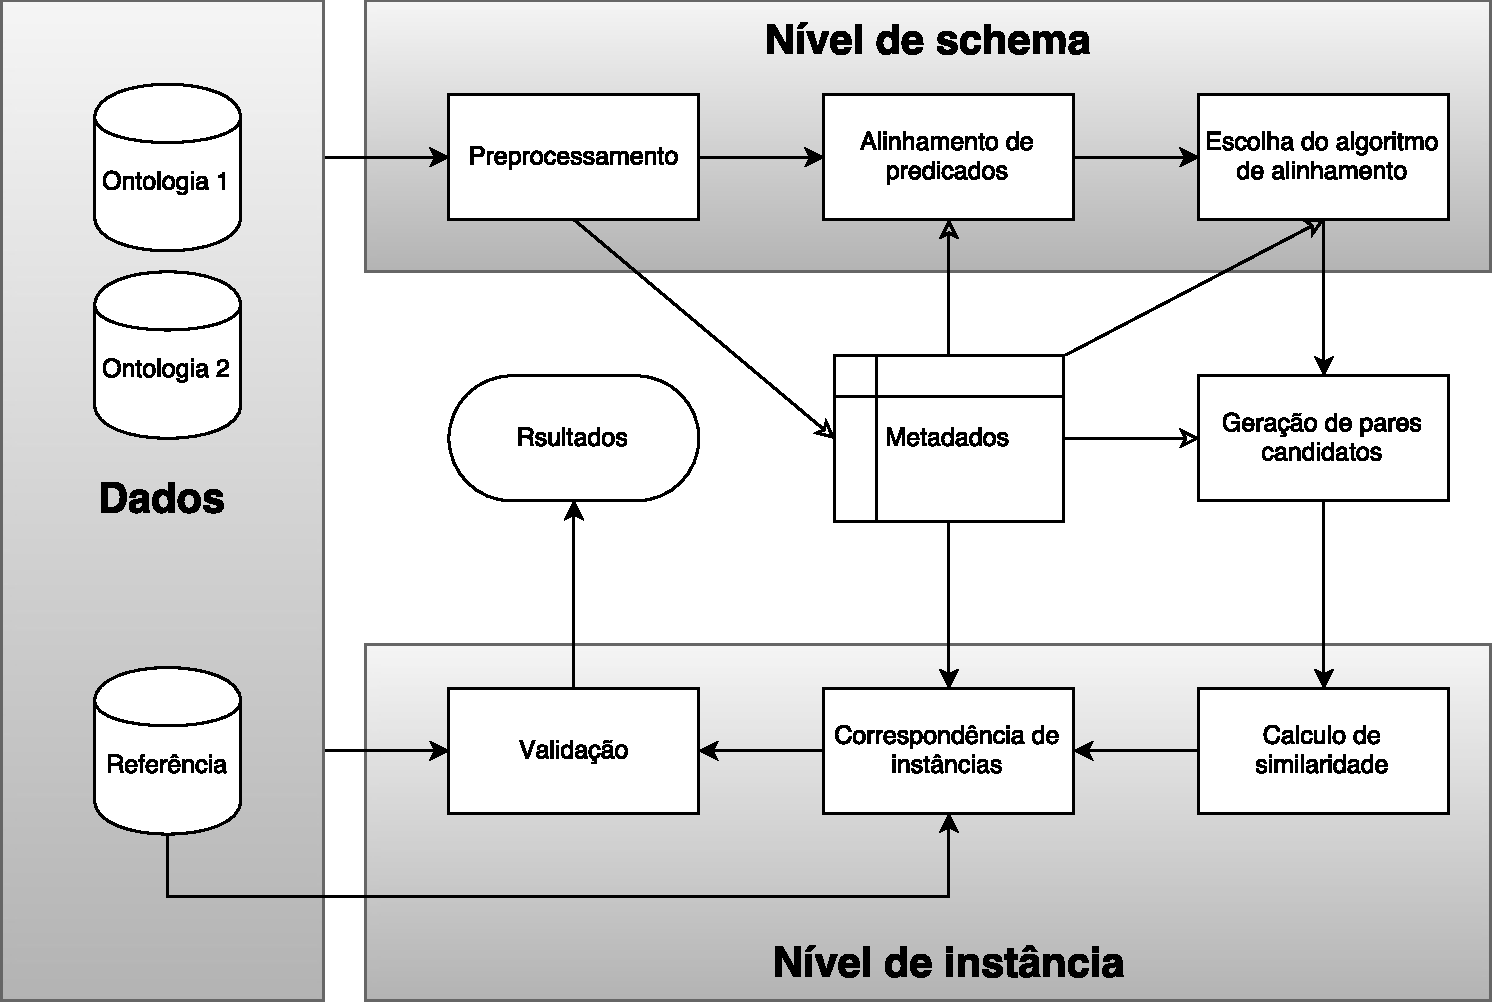
\includegraphics[width=0.8\textwidth]{./imagens/rimom_2016.pdf}
    \caption{Arquitetura do RiMOM-2016}
	\footnotesize{Fonte: adaptado de \cite{zhang2016rimom}}
	\label{fig:rimom}
\end{figure}

Por um lado, o índice invertido permite que um número menor de comparações seja realizado. Por outro lado, a etapa de construção desse índice não considera que os objetos indexados podem conter qualquer tipo de erro. Além disso, como pode ser visto na Figura \ref{fig:rimom}, o RiMOM-2016 utiliza as ontologias apenas para alinhar as propriedades e como entrada para a geração de metadados.

\section{Comparação com a proposta}

Neste capítulo, algumas das principais ferramentas existentes foram apresentadas. Essas ferramentas tem o objetivo de alinhar dados conectados através de diversas abordagens. Dentre os sistemas apresentados, nenhum deles contempla o alinhamento de dados como foco principal, sendo variações de ferramentas existentes para o alinhamento de ontologias.
% * <profsean@gmail.com> 2017-01-18T20:34:14.738Z:
% 
% > nenhum deles contempla o alinhamento de dados como foco principal
% Não tem nenhuma? Será que vc pesquisou direito? Será que não deveria ter buscado ferramentas que fazem alinhamento baseado em instâncias? Se não me engano o pessoal do Marco Antonio Casanova, prof. da PUC-Rio estava trabalhando com isso... não sei se deixaram ferramentas disponíveis. Sugiro dar uma pesquisada porque o Bernardo (que estará na sua banca) foi aluno do Casanova...
% 
% ^.

Esta seção tem o objetivo de apresentar um comparativo entre os trabalhos relacionados e o presente estudo. Para isso, consideramos os seguintes critérios: (1) Quantidade de \textit{datasets} suportados; (2) Tipo de suporte à ontologia; (3) Utilização de computação específica; e (4) Exploração dos conceitos presentes na ontologia.

\begin{table}[h]
	\centering
	\caption{Comparação entre os trabalhos}
	\label{tab:comparacao}
	\begin{tabular}{@{}llll}
		\toprule
		\textbf{Critérios de comparação}                    & \textbf{RiMOM} & \textbf{AML} & \textbf{Proposta} \\ \midrule
		(1) Quantidade de \textit{datasets} suportados    & 2              & 2            & 2+                \\
		(2) Tipo de suporte à ontologia                     & Dirigido       & Dirigido     & Baseado           \\
		(3) Utilização de computação específica             & Sim            & Sim          & Não               \\
		(4) Exploração dos conceitos presentes na ontologia & Não            & Não          & Sim               \\ \bottomrule
	\end{tabular}
\end{table}

Contudo, apesar das ferramentas se mostrarem capazes de encontrar correspondência entre instâncias, ainda deixam a desejar em alguns critérios, tais como a utilização de computação específica para os \textit{datasets}, além da pouca exploração das ontologia, que são utilizadas apenas para a geração de metadados, com o objetivo de escolher entre as abordagens de correspondência disponíveis. Diferentemente das ferramentas citadas, a proposta utiliza ontologias para guiar o processo de correspondência de instância. Além disso, essa abordagem permite que o usuário defina como o alinhamento deve ser realizado.

Outro diferencial da proposta em relação aos trabalhos relacionados está no que chamamos de alinhamento em cascata, que consiste na utilização de instâncias que pertencem a conceitos relacionados ao conceito cujas instâncias serão alinhadas. Ademais, a proposta permite que as correspondências entre as instâncias sejam armazenadas diretamente na base de triplas (\textit{triple store}) em que estão armazenadas.